\documentclass{beamer}
\usepackage[T1]{fontenc}
\usepackage[utf8]{inputenc}

\usetheme{Madrid}
\usecolortheme{default}
\usepackage{amsmath,amssymb,amsfonts,amsthm}
\usepackage{mathtools}
\usepackage{txfonts}
\usepackage{tkz-euclide}
\usepackage{listings}
\usepackage{adjustbox}
\usepackage{array}
\usepackage{gensymb}
\usepackage{tabularx}
\usepackage{gvv}
\usepackage{lmodern}
\usepackage{circuitikz}
\usepackage{tikz}
\lstset{literate={·}{{$\cdot$}}1 {λ}{{$\lambda$}}1 {→}{{$\to$}}1}
\usepackage{graphicx}

\setbeamertemplate{page number in head/foot}[totalframenumber]

\usepackage{tcolorbox}
\tcbuselibrary{minted,breakable,xparse,skins}



\definecolor{bg}{gray}{0.95}
\DeclareTCBListing{mintedbox}{O{}m!O{}}{%
  breakable=true,
  listing engine=minted,
  listing only,
  minted language=#2,
  minted style=default,
  minted options={%
    linenos,
    gobble=0,
    breaklines=true,
    breakafter=,,
    fontsize=\small,
    numbersep=8pt,
    #1},
  boxsep=0pt,
  left skip=0pt,
  right skip=0pt,
  left=25pt,
  right=0pt,
  top=3pt,
  bottom=3pt,
  arc=5pt,
  leftrule=0pt,
  rightrule=0pt,
  bottomrule=2pt,
  toprule=2pt,
  colback=bg,
  colframe=orange!70,
  enhanced,
  overlay={%
    \begin{tcbclipinterior}
    \fill[orange!20!white] (frame.south west) rectangle ([xshift=20pt]frame.north west);
    \end{tcbclipinterior}},
  #3,
}
\lstset{
    language=C,
    basicstyle=\ttfamily\small,
    keywordstyle=\color{blue},
    stringstyle=\color{orange},
    commentstyle=\color{green!60!black},
    numbers=left,
    numberstyle=\tiny\color{gray},
    breaklines=true,
    showstringspaces=false,
}
\title{5.2.13}
\subtitle{System of equation}
\author{EE25BTECH11010 - Arsh Dhoke}
\date{}
\begin{document}


\begin{frame}
  \titlepage
\end{frame}


\begin{frame}{Question}
Solve the following system of linear equations
2x-2y=2 and 4x-4y=5.
\end{frame}

\begin{frame}{Input parameters}
\begin{tabular}{|c|c|}
\hline
\textbf{Name} & \textbf{Value} \\ \hline
$\vec{A}$ & $\myvec{2 & 1 \\0 & 3}$ \\ \hline
\end{tabular}


We can combine and write these 2 equations as
\begin{align}
\myvec{2 & -2 \\ 4 & -4}\myvec{x \\ y} &= \myvec{2 \\ 5}
\end{align}
\end{frame}

\begin{frame}{Gaussian Elimination}
\begin{align}
\augvec{2}{1}{2 & -2 & 2 \\ 4 & -4 & 5} 
\xleftrightarrow{R_2 \rightarrow R_2 - 2R_1} 
\augvec{2}{1}{2 & -2 & 2 \\ 0 & 0 & 1}
\end{align}

The second row shows 0=1 which is a contradiction.


Thus this system is inconsistent with no solution.

\end{frame}

\begin{frame}{Graphical Representation}
\centering
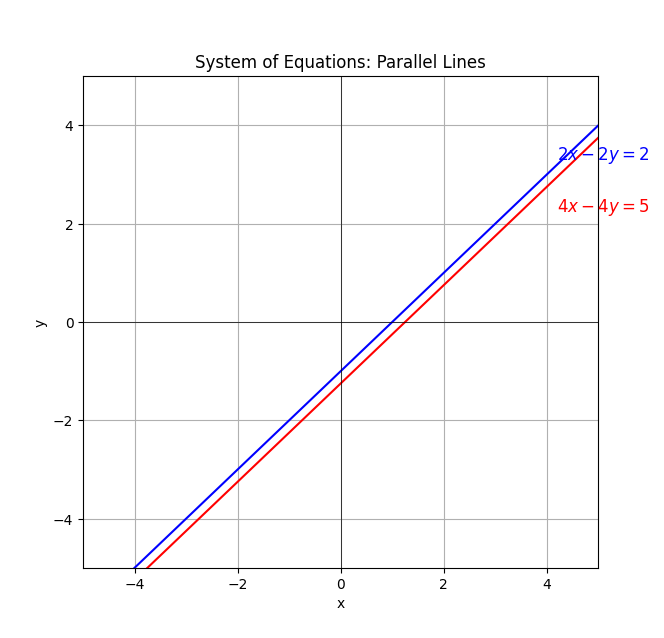
\includegraphics[height=0.7\textheight, keepaspectratio]{figs/q10.png}
 \label{Graph}
\end{frame}

\begin{frame}[fragile]
    \frametitle{C Code}
\begin{lstlisting}
#include<stdio.h>

double eq1(double x) {
    return x - 1.0;
}

double eq2(double x) {
    return x - 1.25;
}
\end{lstlisting}
\end{frame}

\begin{frame}[fragile]
    \frametitle{Python Code}
\begin{lstlisting}
import numpy as np
import matplotlib.pyplot as plt

# Define x range
x = np.linspace(-5, 5, 400)

# Define equations
# Line 1: 2x - 2y = 2 -> y = x - 1
y1 = x - 1
label1 = r'$2x - 2y = 2$'

# Line 2: 4x - 4y = 5 -> y = x - 5/4
y2 = x - 1.25
label2 = r'$4x - 4y = 5$'

# --- Plot lines ---
plt.figure(figsize=(8,8))
line1, = plt.plot(x, y1, color='b')
line2, = plt.plot(x, y2, color='r')
\end{lstlisting}
\end{frame}

\begin{frame}[fragile]
    \frametitle{Python Code}
\begin{lstlisting}
x_coord_1 = 4
y_coord_1 = x_coord_1 - 1
plt.annotate(label1, 
             xy=(x_coord_1, y_coord_1), 
             xytext=(x_coord_1 + 0.2, y_coord_1 + 0.3),
            
             color='b',
             fontsize=12)

x_coord_2 = 4
y_coord_2 = x_coord_2 - 1.25
plt.annotate(label2, 
             xy=(x_coord_2, y_coord_2), 
             xytext=(x_coord_2 + 0.2, y_coord_2 - 0.5), 
             
             color='r',
             fontsize=12)
\end{lstlisting}
\end{frame}


\begin{frame}[fragile]
    \frametitle{Python Code}
\begin{lstlisting}
# --- Standard Plot Setup ---
plt.grid(True)
plt.axhline(0, color='black', linewidth=0.5)
plt.axvline(0, color='black', linewidth=0.5)
plt.xlim(-5, 5)
plt.ylim(-5, 5)

plt.xlabel('x')
plt.ylabel('y')
plt.title('System of Equations: Parallel Lines')
plt.savefig("/home/arsh-dhoke/ee1030-2025/ee25btech11010/matgeo/5.2.13/figs/q10.png")
plt.show()
\end{lstlisting}
\end{frame}

\begin{frame}[fragile]
    \frametitle{Python+ C Code}
\begin{lstlisting}
import ctypes
import numpy as np
import matplotlib.pyplot as plt

# Load shared library
lib = ctypes.CDLL("./code.so")

# Define argtypes and restype for functions
lib.eq1.argtypes = [ctypes.c_double]
lib.eq1.restype = ctypes.c_double

lib.eq2.argtypes = [ctypes.c_double]
lib.eq2.restype = ctypes.c_double

# Generate x values
x_vals = np.linspace(-2, 5, 200)

# Compute y values using C functions
\end{lstlisting}
\end{frame}

\begin{frame}[fragile]
    \frametitle{Python+ C Code}
\begin{lstlisting}
y1_vals = [lib.eq1(float(x)) for x in x_vals]
y2_vals = [lib.eq2(float(x)) for x in x_vals]

# Plot
plt.plot(x_vals, y1_vals, label="2x - 2y = 2")
plt.plot(x_vals, y2_vals, label="4x - 4y = 5")
plt.xlabel("x")
plt.ylabel("y")
plt.title("Graph of the two equations")
plt.legend()
plt.grid(True)
plt.savefig("/home/arsh-dhoke/ee1030-2025/ee25btech11010/matgeo/5.2.13/figs/q10.png")
plt.show()

\end{lstlisting}
\end{frame}
\end{document}